\documentclass[12pt]{report}

\usepackage[margin=1.2in]{geometry}
\usepackage{setspace}
\usepackage{fancyhdr}
\usepackage{multirow}
\usepackage{array}
\usepackage{longtable}
\usepackage{graphicx}
\usepackage{listings}
\usepackage{color}
\usepackage[font=nomarl,labelfont=bf]{caption}


% Header Information
\pagestyle{fancy}
%\fancyhead{}
%\fancyfoot{}
\fancyhead[L]{Fall 2012}
\fancyhead[R]{EE382M - Computer Performance Evaluation and Benchmarking}
\fancyfoot[C]{\thepage}
\renewcommand*\thesection{\arabic{section}}
%\renewcommand{\headrulewidth}{0.4pt}
%\renewcommand{\footrulewidth}{0.4pt}
% END Header Information
\newcommand{\specialcell}[2][c]{%
  \begin{tabular}[#1]{@{}c@{}}#2\end{tabular}}
  
\definecolor{dkgreen}{rgb}{0,0.6,0}
\definecolor{gray}{rgb}{0.5,0.5,0.5}
\definecolor{mauve}{rgb}{0.58,0,0.82}
 
\lstset{ %
  language=Octave,                % the language of the code
  basicstyle=\footnotesize,           % the size of the fonts that are used for the code
  numbers=left,                   % where to put the line-numbers
  numberstyle=\tiny\color{gray},  % the style that is used for the line-numbers
  stepnumber=2,                   % the step between two line-numbers. If it's 1, each line 
                                  % will be numbered
  numbersep=5pt,                  % how far the line-numbers are from the code
  backgroundcolor=\color{white},      % choose the background color. You must add \usepackage{color}
  showspaces=false,               % show spaces adding particular underscores
  showstringspaces=false,         % underline spaces within strings
  showtabs=false,                 % show tabs within strings adding particular underscores
  frame=single,                   % adds a frame around the code
  rulecolor=\color{black},        % if not set, the frame-color may be changed on line-breaks within not-black text (e.g. commens (green here))
  tabsize=2,                      % sets default tabsize to 2 spaces
%  captionpos=b,                   % sets the caption-position to bottom
  breaklines=true,                % sets automatic line breaking
  breakatwhitespace=false,        % sets if automatic breaks should only happen at whitespace
%  title=\lstname,                   % show the filename of files included with \lstinputlisting;
                                  % also try caption instead of title
  keywordstyle=\color{blue},          % keyword style
  commentstyle=\color{dkgreen},       % comment style
  stringstyle=\color{mauve},         % string literal style
  escapeinside={\%*}{*)},            % if you want to add LaTeX within your code
  morekeywords={*,...}               % if you want to add more keywords to the set
}


\newcommand{\Fig}[1]{\figurename~\ref{#1}}
\newcommand{\Figsub}[1]{\figurename~\subref{#1}}
\newcommand{\Tbl}[1]{\tablename~\ref{#1}}
\newcommand{\Sec}[1]{Section~\ref{#1}}

%==========================================================

\begin{document}
%==========================================================

\title{Homework 1: Cache Simulator}
\author{Minsoo Rhu, Jingwen Leng}
\date{Fall 2012}
\maketitle

\section{How to run the cache simulator}

The source files for our cache simulator are listed in \Tbl{src_files}:

\begin{table}[h]
\centering  % used for centering table
\resizebox{\linewidth}{!}{
\begin{tabular}{|c |l| } % centered columns (4 columns)
\hline                        %inserts double horizontal lines
\textbf{Name}  & \textbf{Description} \\ [0.5ex] % inserts table 
\hline \hline
Cache.cpp & \multirow{3}{*}{contains the definition and declarition of Cache class}\\
Cache.h & \\ 
misc.h & \\\hline
main.cpp & main function for multicore cache \\ \hline
singlecache.cpp & main function for single cache \\\hline
autotest.cpp & genrating the trace to test the cache hierachy and paramters. \\\hline
Makefile & make file for cache simulator\\\hline

\hline                  % inserts single horizontal line
\end{tabular}
}
\caption{Source files in our cache simulator} % title of Table
\label{src_files} % is used to refer this table in the text
\end{table}

The make file is going to generate two binaries: \emph{\textbf{cachesim}} and \emph{\textbf{singlecache}}. To run the single cache, use the following command line:

./singlecache 32768 32 2 5 trace-file-name

To run the multi core cache, use the following command line:

./cachesim 4 32 1024 4 4 4 4 trace-file1 trace-file2 trace-file3 trace-file4

The meaning of each parameter is the same as the home work specification.

\subsection{Simulator Output}

\begin{figure}[h]
\lstinputlisting[language=C]{figs/singlecache.output}
\caption{Sample out for single cache.}
\label{fig:singlecache.output}
\end{figure}

\begin{figure}[!h]
%\lstinputlisting[language=C]{figs/multicache.output}
\begin{lstlisting}
[Core-726][L2 Cache][BankId=0][Stats]
- Total Accesses	= 4014
- Total Hits		= 2636
- Total Misses		= 1378
=> Hit  rate		= 0.656702
=> Miss rate		= 0.343298
[Core-726][L2 Cache][BankId=1][Stats]
- Total Accesses	= 4867
- Total Hits		= 3009
- Total Misses		= 1858
=> Hit  rate		= 0.618245
=> Miss rate		= 0.381755
\end{lstlisting}
\caption{Sample out for multi core cache.}
\label{fig:singlecache.output}
\end{figure}

\Fig{fig:singlecache.output} and \Fig{fig:singlecache.output} show the sample output from our cache simulator. The access counts, hit/miss counts and hit/miss ratio are outputed for L1 and L2 cache, as well as for the individual bank in L2. 

%\subsection{T}

\newpage
\section{Description}
\begin{figure}[!h]
\begin{minipage}[b]{\textwidth}
 \centering
 \includegraphics[trim=0mm 0mm 0mm 0mm,clip,width=0.98\linewidth]{figs/cache_structure.pdf}
 \caption{Overall structure of the multi-core cache simulator}
 \label{fig:cache_structure}
\end{minipage}
\end{figure}

\textbf{Single Cache Module.} The core cache module used in our multi-core cache simulator is constructed in a way such that it is easy to debug and re-usable on multiple 
cache-levels (\Fig{fig:cache_structure}(a)). The class structure of a cache module consists of i) a tag-array
class that stores all the necessary information required to track a cache line's state (i.e. tag, line status, accessed time, etc), 
ii) an incoming-access-request-queue structure (using C++ STL containers) that stores cache-access requests from the core (in case of L1D caches) or
the L1D caches (in case of L2D cache), iii) an output-serviced-request-queue structure that spits out serviced request, along with whether
it was a hit/miss, and iv) access-methods that manipulate the cache module (i.e. probe(), access(), send\_serviced\_request, service\_incoming\_request()
and etc). All the abovementioned modules that constitute a cache are structured in a way that operates in a \emph{cycle-level} manner, 
so whenever a single clock cycle is elapsed, an internal \emph{advance\_cycle()} method is called. This method executes the necessary actions that
need to be taken in order to \emph{advance} one clock cycle further, thus allowing the overall cache simulator to not only functionally
emulate the cache, but also to capture the cycle-level behavior. 

\textbf{Multi-Level Cache.} The cache module explained above is used to instantiate a \emph{single} bank amount of hardware that constitutes a cache, so each core instantiates
\emph{one} cache module to mimic its single-bank L1D cache. Accordingly, based on the required specifications of HW1, a total of four banks
are instantiated for L1D caches across the four multi-cores -- note that each banks work independently among each other in L1. Using the same 
cache module, we additionally instantiate \emph{16} cache modules to provide the behavior of the 16-bank L2D cache. Based on how the L2 bank
configuration is selected (i) equally partitioned, ii) unequally partitioned, and iii) shared L2 banks configuration), the \emph{arbiter} coordinates the incoming requests
from L1D to the appropriate L2D banks. As in the cache module, the arbiter also has an \emph{advance\_cycle()} method that enables its cycle-level
behavior.























\newpage
\section{Evaluation}
\subsection{Single Cache}
\label{single_cache}
To test our single cache (core) version of the cache simulator, we generate the memory access trace for program shown in \Fig{fig:autotest}, which uses a fixed stride to access an array (each element is one byte). 

\begin{figure}[ht]
\lstinputlisting[language=C]{figs/autotest.cpp}
\caption{Program to automatically test cache paramters.}
\label{fig:autotest}
\end{figure}

\Fig{fig:autotest_result} shows the results for the program with different array size and stride mentioned previously. We consider this is the signature dictionary of our cache. Next, we are going to explain how to get the cache parameters through the graph. We have also tested the scenario with L2 cache disable, but we only show the results for the single case with both L1 and L2 cache. Parameters for both cache are shown in the Figure.

\begin{figure}[!h]
\begin{minipage}[b]{\textwidth}
 \centering
 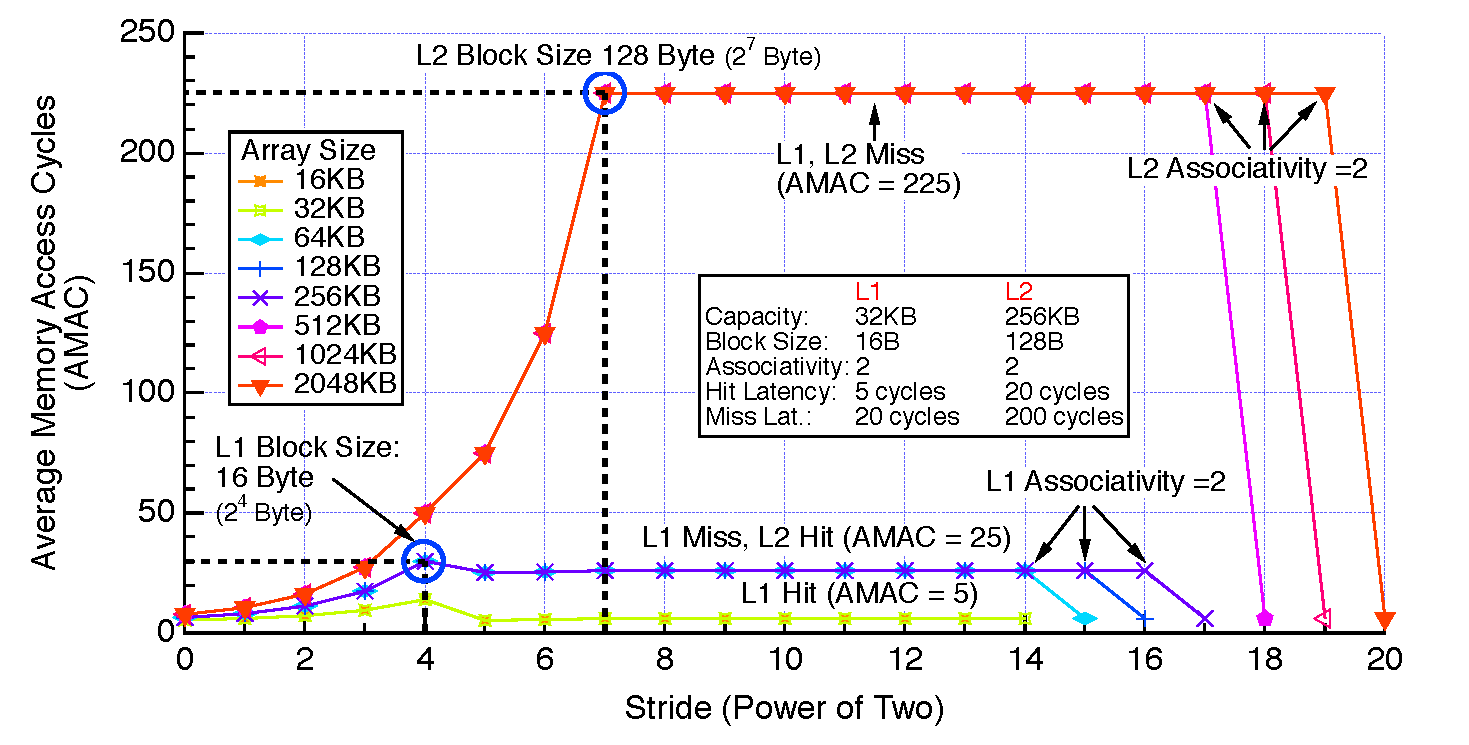
\includegraphics[trim=0mm 0mm 0mm 0mm,clip,width=\linewidth]{figs/autotest.pdf}
 \caption{Average memory access cycles for different array size and stride.}
 \label{fig:autotest_result}
\end{minipage}
\end{figure}

\paragraph{Hit/Miss Latency}
\Fig{fig:autotest_result} shows the average memory access cycles for different scenarios, i.e. L1 hit, L1 miss but L2 hit and L2 miss. The average access cycles for these scenarios are 5, 25 an 225 respectively. 

\paragraph{Cache Capacity}
As shown in the \Fig{fig:autotest_result}, when the array size is 16KB and 32KB, the array size is smaller or equal than the L1 cache capacity (32KB in the Figure). Thus the L1 cache is able to hold the whole array, which result in always L1 hit (except the initial cold miss). Similarly, for array size 64KB, 128KB and 256KB, which are smaller or equal than the L2 capacity 256KB but bigger than the L1 cache capacity, the access is L1 miss but L2 hit. When the array size is bigger than both L1 and L2 size, the memory access will be miss in the L2 cache.

\paragraph{Block Size}
As shown in the \Fig{fig:autotest_result}, when the stride to access memory changes from 8~$(2^3)$~Bytes to 16~$(2^4)$~Bytes, the memory access result in completely L1 miss. This is because the L1 cache block size is 16~Bytes. Access stride bigger than the block size would result in the completely L1 miss. Similarly, the transition point for L2 miss when access stride is 128~$(2^7)$~Bytes matches the L2 cache block size (128~Bytes).

\paragraph{Cache Associativity}
In the \Fig{fig:autotest_result}, when the access stride to access memory changes from $(2^{14})$~Bytes to $(2^{15})$~Bytes at array size 64KB, the memory access changes from L1 miss to L1 hit, although the array size is bigger than the L1 cache size. When the array size is 64KB ($2^{16}$~Bytes) and access stride is $(2^{14})$~Bytes, the program shown in \Fig{fig:autotest} is only accessing four elements in the array (with index 0, 16KB, 32KB and 64KB). However, these addresses have same index and the associativity for L1 cache is 2, each access is suffering conflict miss. When access stride becomes $2^{15}$~Bytes, which is the half size of the array, the program is only accessing two elements in the array. Although they still access the same set in the cache, associativity 2 is enough to guarantee cache his in this scenario. This also applies the array size 128KB and 256KB. For the L2 cache, the transition point for array size 512KB, 1024KB and 2048KB matches the L2 associativity as well.

\subsection{Multicore Cache}

In this homework, the L1 cache is private for each core, thus there is no difference between single core and multi core version. The main difference between these two scenarios come from the L2 cache: it can be equally partitioned, unequally partitioned or shared by all cores. \Sec{single_cache} already focuses on the evaluation of the cache hierarchies. Thus for the multicore cache part, we only focus on the evaluation of different L2 partition/shared cases.

\paragraph{Partitioned L2 Cache}
Typically L2 cache has multiple banks with one read port and one write port to achieve the same effect with a large L2 cache with multiple read/write ports, but with much less area/power overhead. When the L2 cache is partitioned among multiple cores, each core will be assigned with multiple banks that are dedicated to serve that core. The number of L2 cache banks assigned to each core can be equal or unequal. In the partitioned L2 cache, a core is not allowed to access banks assigned to other cores. To validate this property, we first simulate the scenario that four different traces are assigned to four different cores. Then we feed only one trace. (empty traces are fed to other cores)


\begin{table}[t]
\centering  % used for centering table
\resizebox{0.75\linewidth}{!}{
\begin{tabular}{|c| c |c|c|c|c| c| } % centered columns (4 columns)
\hline                        %inserts double horizontal lines
\textbf{Core ID} & \textbf{Bank ID} & \textbf{\specialcell{Four Traces}}  & \textbf{\specialcell{gcc \\ Core 0}} & \textbf{\specialcell{dealII \\ Core 1}} & \textbf{\specialcell{mcf\\Core 2}}& \textbf{\specialcell{soplex\\Core 3}} \\ [0.5ex] % inserts table \hline
\hline
\hline
\multirow{4}{*}{Core 0}&0&4014&4014&0&0&0\\                                                                                        
&1&4867&4867&0&0&0\\ 
&2&4138&4138&1&1&1\\ 
&3&4019&4019&0&0&0\\ \hline
\multirow{4}{*}{Core 1}&4&3926&0&3926&0&0\\ 
&5&4060&0&4060&0&0\\ 
&6&4420&1&4420&1&1\\ 
&7&4028&0&4028&0&0\\ \hline
\multirow{4}{*}{Core 2}&8&20563&0&0&20563&0\\ 
&9&20693&0&0&20693&0\\ 
&10&20616&1&1&20616&1\\ 
&11&20264&0&0&20264&0\\ \hline
\multirow{4}{*}{Core 3}&12&11983&0&0&0&11983\\ 
&13&12914&0&0&0&12914\\ 
&14&12792&1&1&1&12792\\ 
&15&11735&0&0&0&11735\\
\hline                 % inserts single horizontal line
\end{tabular}
}
\caption{L2 bank isolation test.} % title of Table
\label{bank_isolation} % is used to refer this table in the text
\end{table}

\begin{figure}[t]
 \centering
\begin{minipage}[b]{0.8\textwidth}
 \centering
 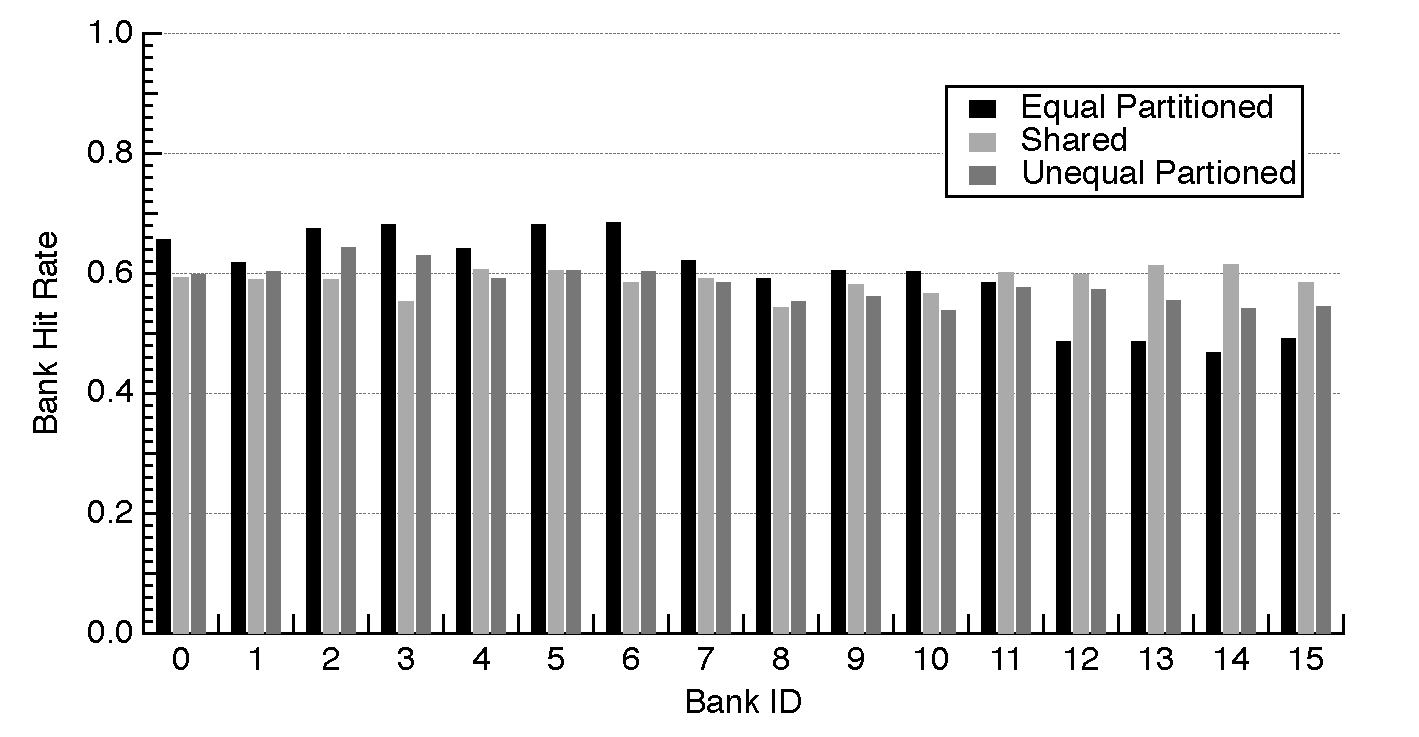
\includegraphics[trim=0mm 0mm 0mm 0mm,clip,width=\linewidth]{figs/bank_hit_rate.pdf}
 \caption{Bank hit rate for different L2 cache scheme.}
 \label{bank_hit}
\end{minipage}
\end{figure}

\Tbl{bank_isolation} shows the result for the bank access isolation test. We used equally partitioned L2 cache for four cores, and each core is assigned with 4 banks. The first two columns of the Table show how banks are assigned to each core. The other columns show the access counts to each bank under different cases. In the \emph{Four Traces} scenario, \emph{gcc} trace is fed to core 0, \emph{dealII} trace is for 1, \emph{mcf} for core 2 and \emph{soplex} for core 3. In the \emph{gcc Core 0} case, gcc trace is fed to core 0 and other cores are fed with a "pseudo" empty trace with only one memory access (that's why other cores have one access in the L2), similarly for other three scenarios. The access counts in \Tbl{bank_isolation} show that in the partitioned case, a core is not able to access other cores' banks.

\paragraph{Shared L2 Cache}
In shared L2 cache, each core is free to access any bank. Here, we compare the metric of \emph{Average Memory Access Time} (AMAT) for the shared L2 cache with partitioned L2 cache.


We used 16-banked L2 cache for 4 cores. The trace fed to each core is the same in the third column of \Tbl{bank_isolation}. \Fig{bank_hit} shows the hit rate for each bank for different schemes. For equal partitioned, we can clearly see core 0 and core 1 have the highest bank hit while core 3 has the lowest hit rate. In the shared L2 cache scheme, each bank has a more evenly distributed bank hit rate. With the knowledge that core 3 has the lowest hit rate, we increase the number of banks assigned to core 3 to 8 (resulting the bank allocation for each core 2 2 4 8, still 16 total banks). The result in \Fig{bank_hit} shows the improvement of bank hit rate for core 3. Core 0 and core 1 are not affected that much since they don not have the desire to a larger cache. 

\begin{figure}[b]
 \centering
\begin{minipage}[b]{0.7\textwidth}
 \centering
 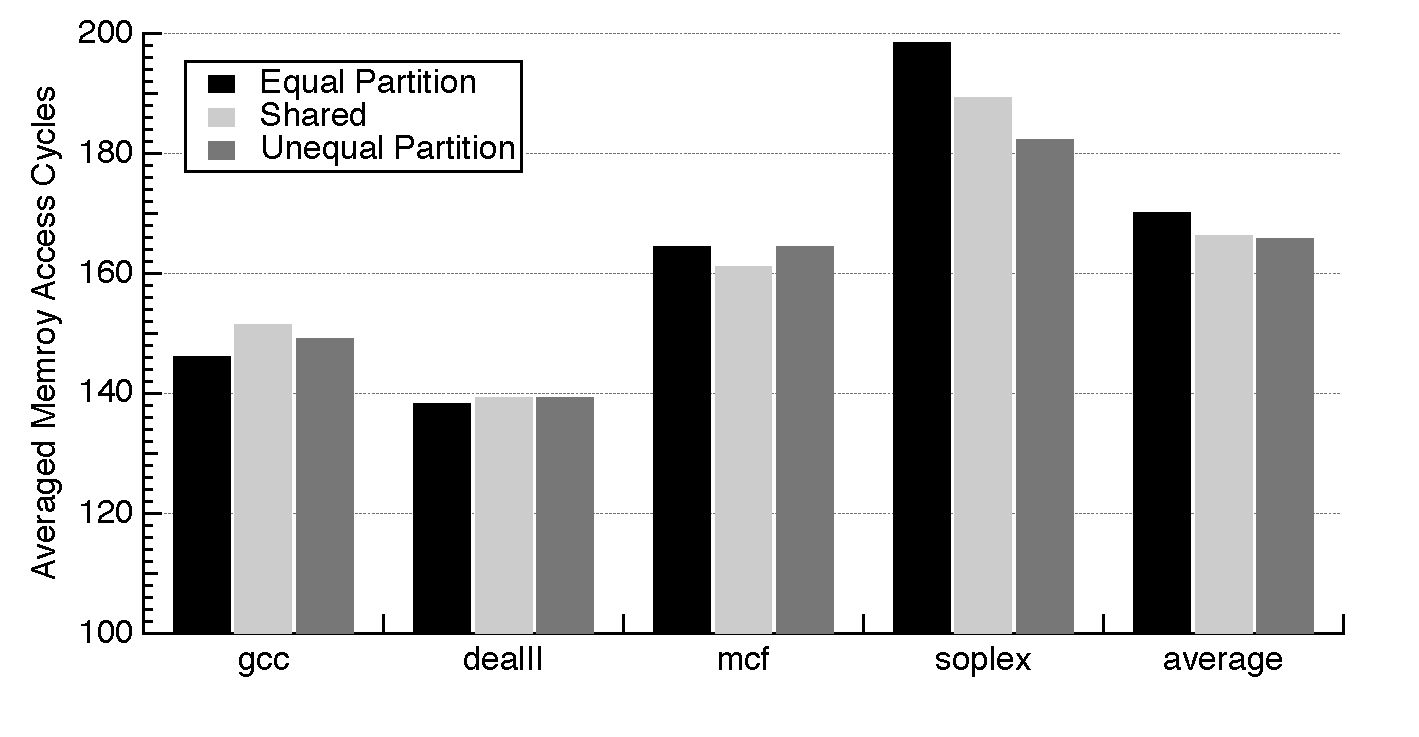
\includegraphics[trim=0mm 0mm 0mm 0mm,clip,width=\linewidth]{figs/bench_stats.pdf}
 \caption{AMAT for different benchmarks.}
 \label{bench_stats}
\end{minipage}
\end{figure}

\Fig{bench_stats} shows the AMAT for each benchmark. We can see the shared L2 cache and the unequal partitioned L2 cache with the knowledge of benchmark characteristics can reduce the AMAT for benchmark \emph{soplex} without affecting other program's performance, resulting a smaller AMAT averaged for these 4 benchmarks.

\end{document}



